\documentclass[12pt]{article}
\usepackage{sammath}

\newcommand{\half}{\frac{1}{2}}
\newcommand{\sixth}{\frac{1}{6}}
\newcommand{\twothird}{\frac{2}{3}}
\newcommand{\dia}[1]{\includegraphics[height=0.7cm]{#1}}

\begin{document}

    \customsection{Overview}

        Work by {\bf Dan Roberts} (FAIR), {\bf Sho Yaida} (FAIR), and {\bf Samuel Tenka} (MIT), 2019.

        We aim to do justice to the stochasticity of the loss landscapes on which gradient methods descend.  
        Thus, in addition to the expectations of the loss, gradient, and hessian, and higher derivatives we also
        consider their variances and higher moments.  Using this data, we Taylor-expand optimizer output with
        respect to the learning rate $\eta$ (i.e. the inverse metric $T^*M \to TM$) to answer questions such as 
        when and why SGD outperforms GD on average, or how well SGD's output generalizes on average.  Our analysis
        applies only when the perturbative series converges quickly, so we validate our predictions empirically.  
        We find that, as predicted, the trace of the covariance of the gradient controls SGD's per-update net
        generalization gap.  We thus propose and demonstrate Stochastic Uncertainty-Repelled Descent (SURD) for quick,
        few-shot learning.  SURD adapts its Taylor-moment estimates as training progresses and is thus robust to 
        the presence of large higher-order Taylor terms.

        \customsubsection{Formal Setting}
            We consider a loss landscape as a flat, complete Riemannian manifold $M$ equipped with a probability
            distribution $S$ of smooth functions on $M$.  We hope in future work to explore relaxations of the flatness
            hypothesis; for example, the natural gradient method of Amari's information geometry operates on 
            a curved manifold, but, as the method's analysis depends on a non-generic relation between Hessian and
            Covariance that is available only on statistical manifolds, we expect our explicit distinction of Hessian
            from Covariance to yield new general insight. 

            {\color{red} TODO Finite moments.}

            The inverse metric $\eta:T^*M \to TM$ will play an especially central role, for it is through this metric
            that we define descent:
            $$
                \theta_{t+1} \leftarrow \theta_t - \eta(\wang{Dl_b}_{b\sim B_t}) 
            $$
            Here, we understand $B_t$ as the $t$th batch.  We model $B_t$ as a loss landscape itself.
            $B_t$ then induces an averaging operation $\wang{\cdot}$.  

        \customsubsection{Prior Work}
            Amari Information Geometry

            Sra Manifold Learning

            Mirror Descent

            Bengio Covariance

            Duchi Variance-Based Regularization

            Nesterov Intro Book

            SGD ``directly optimizes the expected risk'' (e.g. Bottou 2012)



    \customsection{Diagrammatic Expansion of Losses}
        \customsubsection{Use and Interpretation of Diagrams}
            We use diagrams for book-keeping of the Taylor terms (of loss after optimizing from a fixed initial weight). 
            Each color in a diagram represents a data value and thus selects a particular loss function from the
            data-parameterized distribution of loss functions.  Each node in a diagram represents a tensor obtained from
            derivatives of the loss function corresponding to that node's color.  A degree-$d$ node represents a
            $d$th-derivative, contracted with other derivatives as specified by the edges.  A diagram's value is the
            expectation over all iid assigments of data (sampled from $S$) to the colors.  Thus,
            $$
                \dia{rg} := \expec_{\text{red},\text{green}} \nabla^a(l_{\text{red}}) \nabla^a(l_{\text{green}})
                ~~~~~
                \dia{rr} := \expec_{\text{red}} \nabla^a(l_{\text{red}}) \nabla^a(l_{\text{red}})
            $$
            $$
                \dia{rgb} := \expec_{\text{red},\text{green},\text{blue}} \nabla^a(l_{\text{red}}) \nabla^a \nabla^b(l_{\text{green}}) \nabla^b(l_{\text{blue}})
            $$
            $$
                \dia{sgd-2b} := \expec_{\text{red},\text{green},\text{blue}} \nabla^a(l_{\text{red}}) \nabla^b(l_{\text{green}}) \nabla^a \nabla^b(l_{\text{blue}})
            $$
            We see that $\dia{rr}-\dia{rg}$ gives the trace of the covariance of gradients.

            In fact, $\dia{sgd-2a} = \dia{sgd-2b}$, illustrating how diagram notation can streamline computation by
            helping to group terms.  A diagram's value depends on only its topology and its partition into colors, not
            its embedding on a page; $\dia{rggb-a} = \dia{rggb-b} = \dia{new-rgbg}$, for instance.  That said, we
            remember the total order on nodes --- induced by an embedding --- as part of a tree's structure; this
            total order, restricted to the edges, induces a partial order on the nodes. 

        \customsubsection{SGD Test Loss}
            We expand the expected test loss after $T$ updates, each with batch-size $1$ sampled without
            replacement.  The recipe is to draw all the trees whose underlying poset has a unique rightmost element.
            We only count trees whose rightmost element differs from all others in color.  We only count trees
            such that no edge bridges two nodes of the same color and such that the nodes of a given color are
            contiguous in the total ordering on the page.
            Each node in the diagram contributes a factor $1/i!$ where $i$ is the number of edges into the node from
            the left.  Moreover, a diagram with $a$ edges and $v$ vertices has an overall combinatorial weight of
            $(-\eta)^a {T \choose v-1}$.
            \begin{align*}
                \expec \wrap{\text{SGD Test Loss}} = \dia{sgd-0}
                &- \eta   {T \choose 1} \wrap{\dia{sgd-1}} \\
                &+ \eta^2 {T \choose 2} \wrap{\dia{sgd-2a} + \half \dia{sgd-2b}}
                 + \eta^2 {T \choose 1} \wrap{\half \dia{new-rrg}} \\
                &- \eta^3 {T \choose 3} \wrap{\substack{
                        \dia{sgd-3a} + \half \dia{sgd-3b} + \half \dia{sgd-3c} + \\
                        \half \dia{sgd-3d} + \half \dia{sgd-3e} + \sixth \dia{sgd-3f}
                        }} \\  
                &- \eta^3 {T \choose 2} \wrap{\substack{
                        \dia{new-rggb} + \half \dia{new-rrgb-a} + \\
                        \frac{2}{6} \dia{new-rrgb-b} + \frac{2}{2} \dia{new-rrgb-c}
                        }} \\ 
                &- \eta^3 {T \choose 1} \wrap{\sixth \dia{new-rrrg}} 
                 + o(\eta^3)
            \end{align*}
            And a routine grouping of terms yields:
            \begin{align*}
                \cdots = \dia{sgd-0}
                &- \eta   {T \choose 1} \wrap{\dia{sgd-1}} \\
                &+ \eta^2 {T \choose 2} \wrap{\frac{3}{2}\dia{sgd-2a}}
                 + \eta^2 {T \choose 1} \wrap{\half \dia{new-rrg}} \\
                &- \eta^3 {T \choose 3} \wrap{\frac{5}{2} \dia{sgd-3a} + \twothird \dia{sgd-3b}} \\
                    &- \eta^3 {T \choose 2} \wrap{\dia{new-rggb} + \frac{5}{6} \dia{new-rrgb-a} + \dia{new-rrgb-c}} \\
                &- \eta^3 {T \choose 1} \wrap{\sixth \dia{new-rrrg}} 
                 + o(\eta^3)
            \end{align*}

        \customsubsection{Variants: GD, Train Loss, Multiepoch}
            To compute losses for (non-stochastic) gradient descent, we allow non-rightmost nodes to share colors with
            each other.
            To compute train losses, we allow the rightmost node to share a color with previous nodes with probability
            $C/N$, where $C$ counts the non-rightmost colors in the diagram. 
            The multiepoch case has a similar analysis; for SGD test loss:
            $$
                \text{SGD}(\eta, T, E) = \text{SGD}(E\eta, T, 1) + \eta^2 {T \choose 1} {E \choose 2} \dia{new-rrg} + o(\eta^2)  
            $$
            Subtracting, we compute generalization gaps, the benefit of stochasticity, and the effect of epochs.

            {\color{red} TODO We now give the explicit forms.}


    \customsection{Intepretation of Terms}
        \customsubsection{Trace-Covariance as Problem Complexity}
            Consider the classic problem of least-squares mean estimation in dimension $d$.  If the true distribution
            has covariance $C$, then so will the gradient $D_w l_x = D_w(\|w-x\|^2/2) = (w-x)^T$.  Intuitively, the
            trace of this covariance, normalized by the largest singular value, is a smooth bound on the data's
            dimension, for if $x$ lies in a vector subspace of dimension $c\leq d$, then $\text{tr}(C) / \|C\| \leq c$.
            When the data distribution is $\sigma^2$-subgaussian, this trace controls generalization of the na\"ive
            estimator, for the empirical mean on $N$ iid points differs from the true mean
            by (a multiple of $\sigma^2/N$, a scalar summary of $\hat x$'s spread):
            $$
                \expec\wive{\|\hat x - \mu\|^2} \leq \frac{\sigma^2}{N} \frac{\text{tr}(C)}{\|C\|}
            $$

            Motivated by this connection between $\text{tr}(C)/\|C\|$ and dimension in the special context of least-squares
            mean estimation, as well as the connection between $\text{tr}(C)$ and generalization complexity in our preceding 
            analysis of gradient methods, we define the {\bf local dimension} of a loss landscape for each
            $w\in M$:
            $$
                \text{dim}(w) := \frac{\text{tr}(C(w))}{\|C(w)\|} \in [0, \text{dim}(M)]
            $$

            The normalization by $\|C\|$ ensures that $\text{dim}(w)$ measures the effective dimension of SGD's 
            updates in a way invariant to scalings of batch size or learning rate.  We may test the degree to which
            SGD's established avoidance of high-$\text{tr}(C)$ regions translates to an avoidance of
            high-$\text{dim}(w)$ regions.  For example, consider a toy loss landscape of form
            $$
                l_x(w) = \wrap{(w - x)^2 - (1-x)^2}^2 
            $$
            {\color{red} TODO example plots for toy and also for section of MNIST deep.
             Illustrate how {\bf saturation} and {\bf correlations} of hidden activations lead to lower effective dimension} 

        \customsubsection{Bounds for Neglected Terms in Logistic Regression}
            {\color{red} TODO}

    \customsection{Empirics}
        \customsubsection{SGD for MNIST Binary Classification}
            \begin{figure}[h]
                \center
                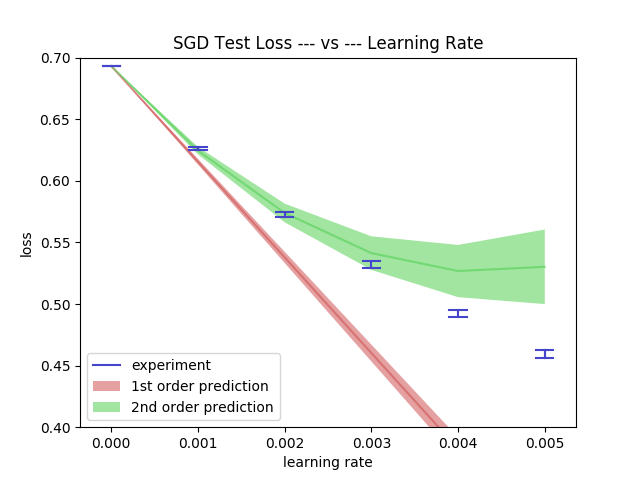
\includegraphics[width=5.25cm]{out-sgd-logis}
                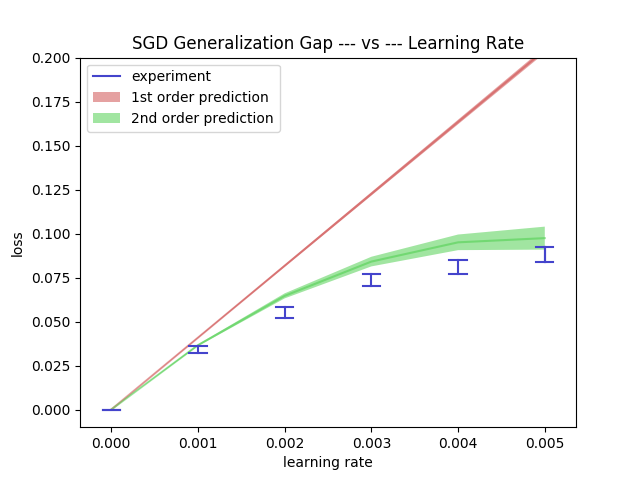
\includegraphics[width=5.25cm]{gen-sgd-logis}
                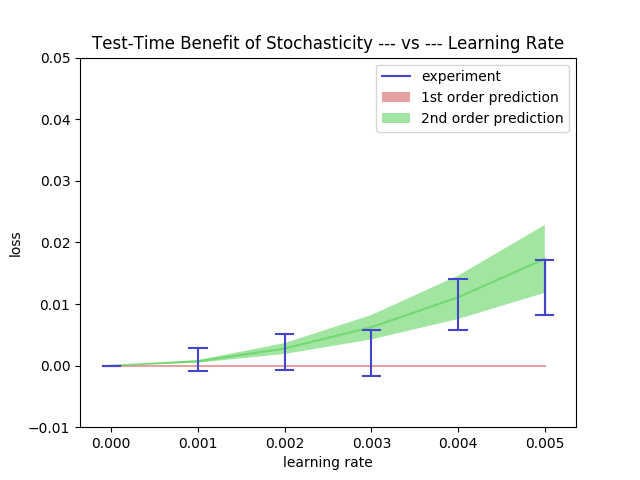
\includegraphics[width=5.25cm]{out-diff-logis}
                \caption{
                    Logistic Regression for $N=T=100$.
                    {\bf Left}: For SGD test loss, larger learning rates give diminishing returns.
                    {\bf Middle}: Covariance indeed predicts SGD generalization gap.
                    {\bf Right}: SGD outperforms GD, as predicted by covariance data.
                    }
            \end{figure}

            \begin{figure}[h]
                \center
                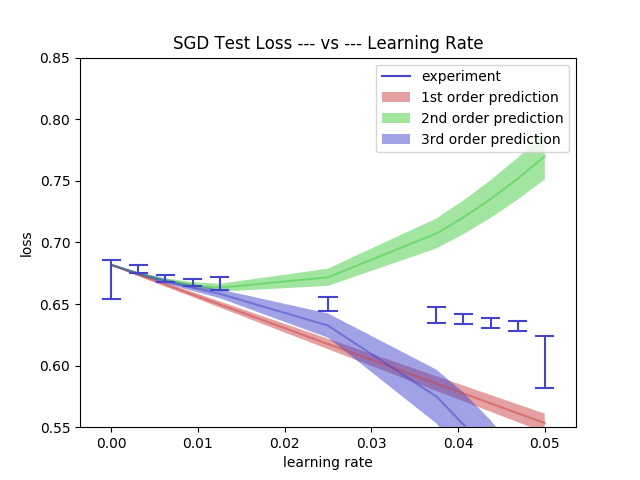
\includegraphics[width=5.25cm]{out-sgd-deep17}
                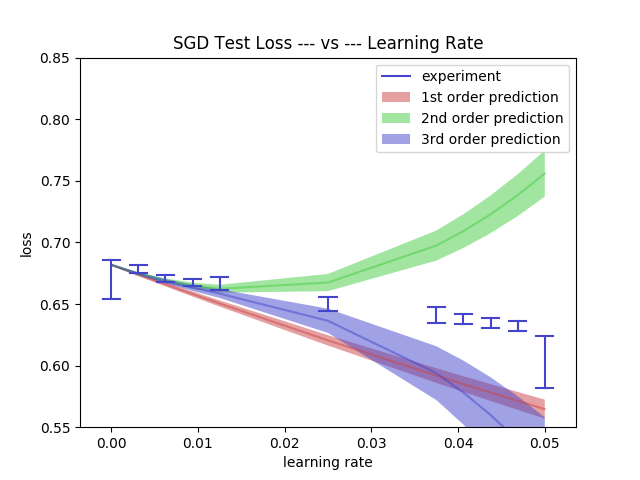
\includegraphics[width=5.25cm]{out-sgd-deep17-exp}
                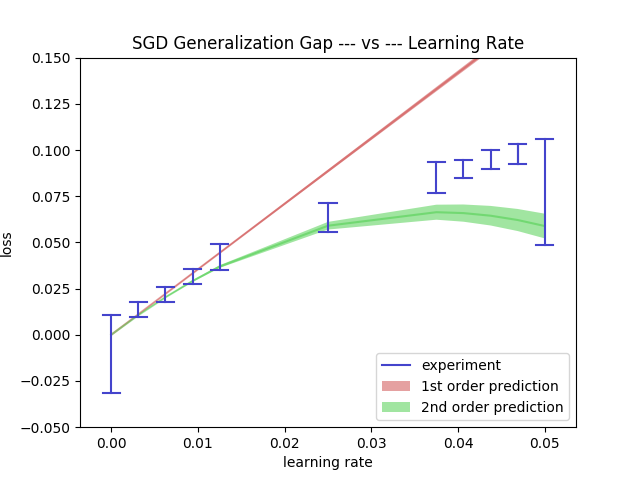
\includegraphics[width=5.25cm]{gen-sgd-deep17}
                \caption{
                    Neural Network (two tanh hidden layers of size 25) for $N=T=10$.
                    We trained faster (in the wee hours before Sasha's group meet) by cutting
                    each MNIST image to just its 14th column.  This reduces 784 features to 28 features.  
                    {\bf Left}: SGD test loss, polynomial approximation --- bad fit.
                    {\bf Middle}: SGD test loss, exponential approximation --- bad fit.
                    {\bf Right}: SGD generalization gap --- good fit, perhaps because higher-order terms cancel. 
                    }
            \end{figure}

        \customsubsection{Variance and Gradient-Covariance for Regularization}


\end{document}
